\documentclass[12pt]{article}
\newif\ifblind
\blindfalse
% \blindtrue
% Common preamble of wellbeing.tex, wellbeing_region.tex and wellbeing_discrepancy.tex
% Compile from papers/:  latexmk -pdf -outdir=build <file>.tex
\usepackage[T1]{fontenc}
\usepackage[utf8]{inputenc}
\usepackage{lmodern}
\usepackage[margin=2.5cm]{geometry}
\usepackage{setspace}
\onehalfspacing
\usepackage{amsmath, amssymb}
\usepackage{graphicx}
\usepackage{booktabs, makecell, threeparttable, adjustbox}
\usepackage{caption}
\captionsetup{font=small, labelfont=bf}
\usepackage[authoryear, round]{natbib}
\bibliographystyle{apalike}
\usepackage{xspace}
\usepackage{xcolor}
\usepackage[colorlinks=true, linkcolor=blue!60!black, citecolor=blue!60!black, urlcolor=blue!60!black]{hyperref}
\usepackage{lineno}
% Placeholders for information to be completed by the author
\newcommand{\todo}[1]{\textcolor{red}{[TODO: #1]}}
% Numbers computed by code_wellbeing/main.R (percentages are given without the % sign)
\newcommand{\corGallupWHR}{0.993\xspace}
\newcommand{\corGallupWHRoldMapping}{0.89\xspace}
\newcommand{\nGallupCountryYears}{2351\xspace}
\newcommand{\nGallupCountries}{168\xspace}
\newcommand{\nWVSCountryYears}{304\xspace}
\newcommand{\nWVSCountries}{108\xspace}
\newcommand{\nWVSRespondents}{439531\xspace}
\newcommand{\nFabre}{11000\xspace}
\newcommand{\nFabreCountries}{10\xspace}
\newcommand{\bestIncome}{Cluster k=7 nominal\xspace}
\newcommand{\shareRegionBetterWVS}{86\xspace}
\newcommand{\shareRegionBetterWVSbest}{79\xspace}
\newcommand{\nSpecsWVS}{952\xspace}
\newcommand{\meanShareIncomeBest}{28\xspace}
\newcommand{\meanRtwoIncomeBest}{19\xspace}
\newcommand{\meanRtwoIncomePPP}{12\xspace}
\newcommand{\meanRtwoRegion}{37\xspace}
\newcommand{\RtwoSatisfiedMeanPPP}{20\xspace}
\newcommand{\RtwoHappinessMeanPPP}{4\xspace}
\newcommand{\RtwoVeryHappyPPP}{0\xspace}
\newcommand{\shareRegionBetterGallup}{35\xspace}
\newcommand{\shareIncomeGallupMean}{60\xspace}
\newcommand{\RtwoGallupMeanPPP}{61\xspace}
\newcommand{\RtwoGallupRegion}{48\xspace}
\newcommand{\RtwoWHRPPP}{63\xspace}
\newcommand{\RtwoWHRRegion}{55\xspace}
\newcommand{\shareRegionBetterNoLatamEE}{27\xspace}
\newcommand{\shareIncomeNoLatamEE}{34\xspace}
\newcommand{\shareRegionBetterContinents}{54\xspace}
\newcommand{\shareRegionBetterWB}{64\xspace}
\newcommand{\cvIncomeSatisfiedMean}{0.18\xspace}
\newcommand{\cvRegionSatisfiedMean}{0.44\xspace}
\newcommand{\cvIncomeGallupMean}{0.60\xspace}
\newcommand{\cvRegionGallupMean}{0.45\xspace}
\newcommand{\shareCvRegionBetterWVS}{100\xspace}
\newcommand{\corHappySatisfied}{0.72\xspace}
\newcommand{\corHappinessSatisfactionMean}{0.76\xspace}
\newcommand{\corVeryHappySatisfiedMean}{0.63\xspace}
\newcommand{\slopeVeryHappy}{0.005\xspace}
\newcommand{\pVeryHappy}{0.85\xspace}
\newcommand{\happiestFirst}{Switzerland\xspace}
\newcommand{\happiestFirstN}{10\xspace}
\newcommand{\happiestSecond}{Mexico\xspace}
\newcommand{\happiestSecondN}{9\xspace}
\newcommand{\happiestThird}{Kyrgyzstan\xspace}
\newcommand{\happiestThirdN}{6\xspace}
\newcommand{\happiestRegionWestern}{24\xspace}
\newcommand{\happiestRegionLatinAmerica}{19\xspace}
\newcommand{\happiestRegionAsia}{16\xspace}
\newcommand{\happiestRegionAfrica}{5\xspace}
\newcommand{\nHappiestCells}{64\xspace}
\newcommand{\treeRegionFirst}{8\xspace}
\newcommand{\withinRtwoSatisfiedMean}{0.22\xspace}
\newcommand{\withinSlopeSatisfiedMean}{1.68\xspace}
\newcommand{\crossSlopeSatisfiedMean}{1.09\xspace}
\newcommand{\withinSlopeVeryHappy}{0.18\xspace}
\newcommand{\pWithinVeryHappy}{0.004\xspace}
\newcommand{\nWithin}{272\xspace}
\newcommand{\RtwoFreedomSatisfaction}{63\xspace}
\newcommand{\shapleyFreedom}{40\xspace}
\newcommand{\shapleyFreedomRegion}{26\xspace}
\newcommand{\shapleyFreedomIncome}{9\xspace}
\newcommand{\RtwoTolerance}{21\xspace}
\newcommand{\RtwoGod}{0\xspace}
\newcommand{\RtwoGrowth}{2\xspace}
\newcommand{\nonresponseSatisfactionWVS}{1.5\xspace}
\newcommand{\nonresponseHappinessWVS}{1.7\xspace}
\newcommand{\corNonresponseGDP}{-0.08\xspace}
\newcommand{\effectLadder}{-0.45\xspace}
\newcommand{\seLadder}{0.05\xspace}
\newcommand{\effectScale}{0.14\xspace}
\newcommand{\seScale}{0.05\xspace}
\newcommand{\effectLadderZeroTen}{-0.46\xspace}
\newcommand{\effectScaleZeroTen}{-0.26\xspace}
\newcommand{\effectLadderSatisfied}{-9\xspace}
\newcommand{\interactionLadderIncome}{-0.004\xspace}
\newcommand{\pInteractionLadderIncome}{0.92\xspace}
\newcommand{\gradientIncomeSatisfaction}{0.69\xspace}
\newcommand{\pHeterogeneityWording}{0.000\xspace}
\newcommand{\chiHeterogeneityWording}{93.4\xspace}
\newcommand{\wordingCHE}{-0.34\xspace}
\newcommand{\wordingDEU}{-0.53\xspace}
\newcommand{\wordingESP}{-1.12\xspace}
\newcommand{\wordingFRA}{-0.50\xspace}
\newcommand{\wordingGBR}{-0.63\xspace}
\newcommand{\wordingITA}{-0.55\xspace}
\newcommand{\wordingJPN}{0.36\xspace}
\newcommand{\wordingPOL}{-0.55\xspace}
\newcommand{\wordingSAU}{-0.79\xspace}
\newcommand{\wordingUSA}{-0.63\xspace}
\newcommand{\wordingMin}{-1.12\xspace}
\newcommand{\wordingMax}{0.36\xspace}
\newcommand{\decompMeanGap}{-0.39\xspace}
\newcommand{\decompMeanQuestion}{-0.71\xspace}
\newcommand{\decompMeanResidual}{0.32\xspace}
\newcommand{\decompShareLevelQuestion}{1.83\xspace}
\newcommand{\decompVarShareQuestion}{-0.20\xspace}
\newcommand{\decompVarShareResidual}{1.20\xspace}
\newcommand{\decompMeanAbsGap}{0.43\xspace}
\newcommand{\decompMeanAbsResidual}{0.64\xspace}
\newcommand{\decompRmsePredictionGallup}{0.73\xspace}
\newcommand{\decompRmseNaive}{0.42\xspace}
\newcommand{\decompMeanGapSat}{-0.05\xspace}
\newcommand{\decompMeanQuestionSat}{-0.11\xspace}
\newcommand{\decompVarShareQuestionSat}{-0.11\xspace}
\newcommand{\decompSdGap}{0.44\xspace}
\newcommand{\decompSdQuestion}{0.45\xspace}
\newcommand{\decompSdResidual}{0.69\xspace}
\newcommand{\decompCorGapQuestion}{-0.20\xspace}
\newcommand{\decompLowMeanGap}{-0.44\xspace}
\newcommand{\decompHighMeanGap}{-0.34\xspace}
\newcommand{\decompLowMeanQuestion}{-0.85\xspace}
\newcommand{\decompHighMeanQuestion}{-0.56\xspace}
\newcommand{\decompLowMeanResidual}{0.17\xspace}
\newcommand{\decompHighMeanResidual}{0.46\xspace}
\newcommand{\decompLowVarShareQuestion}{-0.52\xspace}
\newcommand{\decompHighVarShareQuestion}{0.15\xspace}
\newcommand{\decompLowShareLevelQuestion}{1.42\xspace}
\newcommand{\decompHighShareLevelQuestion}{2.27\xspace}
\newcommand{\decompLowCorGapQuestion}{-0.47\xspace}
\newcommand{\decompHighCorGapQuestion}{0.14\xspace}
\newcommand{\nDecompCountries}{10\xspace}
\newcommand{\nSameYear}{7\xspace}
\newcommand{\nRecent}{4\xspace}
\newcommand{\varShareQuestionSameYear}{-0.27\xspace}
\newcommand{\varShareQuestionRecent}{-0.81\xspace}
\newcommand{\shareLevelQuestionSameYear}{1.60\xspace}
\newcommand{\shareLevelQuestionRecent}{1.19\xspace}
\newcommand{\meanSampleEffectGallup}{0.75\xspace}
\newcommand{\corFabreWHR}{0.75\xspace}
\newcommand{\minSampleEffectGallup}{0.16\xspace}
\newcommand{\maxSampleEffectGallup}{1.24\xspace}
\newcommand{\meanSampleEffectWVS}{0.54\xspace}
\newcommand{\meanFabreGallupZero}{5.93\xspace}
\newcommand{\meanFabreWVSOne}{6.64\xspace}
\newcommand{\sampleEffectUSWVS}{0.49\xspace}
\newcommand{\nCommon}{149\xspace}
\newcommand{\nCommonCountries}{83\xspace}
\newcommand{\RtwoCommonGallup}{0.49\xspace}
\newcommand{\RtwoCommonWVS}{0.11\xspace}
\newcommand{\slopeCommonGallup}{1.76\xspace}
\newcommand{\slopeCommonWVS}{0.77\xspace}
\newcommand{\slopeGapGDP}{1.07\xspace}
\newcommand{\seSlopeGapGDP}{0.16\xspace}
\newcommand{\RtwoGapGDP}{0.31\xspace}
\newcommand{\slopeQuestionGDP}{0.30\xspace}
\newcommand{\seSlopeQuestionGDP}{1.75\xspace}
\newcommand{\RtwoAdjustedWVS}{0.20\xspace}
\newcommand{\shareIncomeCommonGallup}{51\xspace}
\newcommand{\shareIncomeCommonWVS}{15\xspace}

\newcommand{\Rsq}{\ensuremath{R^2}\xspace}
% Switch: show region-specific material (set to false in wellbeing_discrepancy.tex)
\newif\ifshowregion
\showregiontrue

\showregionfalse
% Split paper 2: is the Gallup/WVS discrepancy due to question wording or to samples? (max. 9,000 words excluding appendices)
% Compile from papers/:  latexmk -pdf -outdir=build wellbeing_discrepancy.tex

\title{Ladder or Satisfaction? Why Gallup and the World Values Survey\\ Disagree on Income and Well-Being\thanks{Data and code: \url{https://github.com/bixiou/wellbeing_gdp_region} \todo{public repository (e.g.\ OSF); Gallup data cannot be redistributed}. The survey was approved by the CIRED institutional review board (IRB-CIRED-2025-2) and pre-registered at \href{https://osf.io/7mzn4}{osf.io/7mzn4}. I thank Claudia Senik and participants in the 2024 STATEC Well-being Conference for helpful comments, Armon Rezai and the Vienna University of Economics and Business (WU Wien) for access to the Gallup World Poll data, and Julieta Toffoli for research assistance. This research did not receive any specific grant from funding agencies in the public, commercial, or not-for-profit sectors. Declaration of interest: none.}}
\author{Adrien Fabre\\ \small CNRS, CIRED \todo{postal address}\\ \small \href{mailto:adrien.fabre@cnrs.fr}{adrien.fabre@cnrs.fr}}
\date{\today}

\begin{document}
\maketitle

\begin{abstract}
\noindent The two main sources of cross-national data on subjective well-being disagree: life evaluations are much more strongly related to GDP per capita in the Gallup World Poll (Cantril ladder, 0--10) than in the World Values Survey (WVS; life satisfaction, 1--10), here complemented with the European Values Study. In \nCommon country-years observed by both, log GDP per capita explains \RtwoCommonGallup of the variance of Gallup's mean ladder but \RtwoCommonWVS of WVS mean satisfaction. Is this due to the question or to the samples? I randomize the wording (ladder vs.\ satisfaction) and the scale (0--10 vs.\ 1--10) in an online survey of \nFabre respondents in ten high-income countries. Asked to the same sample, the ladder is better predicted by GDP than the satisfaction question ($R^2$ of \RtwoTenFabreLadderPooled vs.\ \RtwoTenFabreSatisfactionPooled across countries), which reproduces about half of the Gallup--WVS difference in predictive capacity in these countries (\RtwoTenGallup vs.\ \RtwoTenWVS): the new data lie midway between Gallup and the WVS. But both questions yield income gradients as steep as Gallup's, three times steeper than the WVS's: the satisfaction question adds country-specific dispersion, while the flat WVS gradient is specific to its samples. The ladder also shifts answers by \effectLadder points, which fully accounts for Gallup's lower average level, but not for the cross-country pattern of the gap.
\end{abstract}

\noindent\textbf{Keywords:} subjective well-being; life satisfaction; Cantril ladder; question wording; survey mode; survey experiment.\\
\noindent\textbf{JEL codes:} I31; C83; C90.

% \linenumbers
\section{Introduction}\label{sec:intro}

Cross-country comparisons of subjective well-being rely mostly on two surveys: the Gallup World Poll, which underlies the World Happiness Report, and the World Values Survey (WVS). They measure life evaluation with different questions. Gallup asks respondents to place themselves on a ladder whose top represents ``the best possible life for you'' \citep{cantril_pattern_1965}, on a scale from 0 to 10; the WVS (and the European Values Study, EVS, which asks the same question) asks ``how satisfied are you with your life as a whole these days?'', on a scale from 1 to 10. They also differ in their samples: sampling frames, interview modes, questionnaire context, translations, and the years in which each country is surveyed.

The two surveys paint different pictures of the relationship between income and well-being. \citet{deaton_income_2008} documented that Gallup's ladder is strongly related to GDP per capita, more so than WVS measures. The difference is large: in the \nCommon country-years (\nCommonCountries countries) observed by both surveys the same year, log GDP per capita explains \RtwoCommonGallup of the variance of Gallup's mean ladder, but only \RtwoCommonWVS of WVS mean satisfaction. Conclusions on whether ``money buys happiness'' across countries, or on whether a country's world region predicts well-being better than its income, depend on which survey one uses. \todo{cite companion paper on region vs.\ income.}

Which difference is responsible: the question, or the samples? If the question, then the two surveys measure different constructs---for instance, if the ladder elicits thoughts about wealth and status \citep{nilsson_cantril_2024} or evaluative rather than hedonic judgments \citep{kahneman_high_2010}---and multiple indicators should be used. If the samples, then the surveys measure the same construct with different errors, and one should favor the dataset with the most reliable and comparable samples. Observational comparisons cannot answer this question, because the question and the sample always differ together \citep{bjornskov_how_2010}.

I answer it with a survey experiment. In an online survey of \nFabre respondents in ten high-income countries \citep{fabre_public_2025}, I randomly assigned respondents to one of four versions of the life-evaluation question, crossing the wording (Gallup's ladder vs.\ WVS life satisfaction) with the scale (0--10 vs.\ 1--10). The experiment estimates the question effect holding the sample constant. Combining it with Gallup and WVS data for the same countries, I decompose the observed Gallup--WVS gap into a question effect and a residual that captures differences between samples in a broad sense.

The results are nuanced. Asked to the same sample, the two questions reproduce much of the difference in predictive capacity between Gallup and the WVS: across the ten countries, log GDP per capita explains \RtwoTenFabreLadderPooled of the variance of the mean ladder but \RtwoTenFabreSatisfactionPooled of mean satisfaction, compared with \RtwoTenGallup and \RtwoTenWVS in Gallup and the WVS. The wording thus accounts for about half (\decompShareRWordingPooled) of the Gallup--WVS difference in $R^2$, and the new data lie midway between the two datasets. However, the income gradient is similar with both questions (slopes of \slopeTenFabreLadderPooled and \slopeTenFabreSatisfactionPooled on $\log_{10}$ GDP per capita), close to Gallup's (\slopeTenGallup) and three times steeper than the WVS's (\slopeTenWVS): the satisfaction question produces larger country-specific deviations from the income gradient, while the flat WVS gradient is specific to its samples. The question also matters for levels: the ladder shifts answers by \effectLadder points on average, which more than accounts for the lower level of Gallup data in these countries, but explains little of the cross-country variation of the gap. The experiment covers only high-income countries, so it cannot exclude a larger wording effect in poorer countries, where the gap between the two surveys is largest.

The paper contributes to the methodological literature on the measurement of subjective well-being \citep{kahneman_developments_2006,oecd_guidelines_2013,stone_subjective_2013,kaiser_scientific_2022}, in particular on question and scale effects \citep{conti_survey_2011,bond_sad_2019}, context effects \citep{deaton_financial_2012,deaton_understanding_2016}, and mode effects \citep{dolan_happy_2016}, and to the debate on the cross-country relation between income and well-being \citep{deaton_income_2008,stevenson_economic_2008,sacks_new_2012}.

\section{Data}\label{sec:data}
% Shared section: data on national well-being, income and regions (WVS, Gallup, WHR, WDI)
\subsection{World Values Survey}\label{subsec:wvs}

The World Values Survey (WVS) is the longest-running cross-national survey of values and subjective well-being. I use the WVS time-series file \citep{wvs_trend_2022}, which pools the seven waves conducted between 1981 and 2022, and complete it with the Joint EVS/WVS 2017--2022 dataset \citep{evs_wvs_joint_2024}, which adds the \nEVSSurveys national surveys of the 2017 wave of the European Values Study (EVS, conducted in 2017--2021) and \nNewWVSSurveys recent WVS surveys (India 2023, Uzbekistan 2022). The EVS asks the same well-being questions, and the combination of the two surveys is standard practice (the so-called Integrated Values Surveys). The EVS and the WVS are distinct surveys: when both surveyed the same country the same year (\nEVSSameYearWVS cases), I keep both surveys as separate observations.
For brevity, I refer to the combined data as the WVS: \nWVSRespondents respondents in \nWVSCountryYears country-years and \nWVSCountries countries. National samples are designed to be representative of the adult population, typically with 1,000 to 3,000 respondents, and most interviews are conducted face-to-face (though some recent national surveys used web, mail or mixed modes, e.g.\ the WVS in the United States in 2017 and in Japan in 2019, or the EVS in Switzerland in 2017). All statistics use the survey weights provided by the WVS and the EVS.

The WVS contains two questions on subjective well-being:
\begin{itemize}
    \item \textit{Happiness}: ``Taking all things together, would you say you are: \textit{Very happy}; \textit{Quite happy}; \textit{Not very happy}; \textit{Not at all happy}.''
    \item \textit{Life satisfaction}: ``All things considered, how satisfied are you with your life as a whole these days?'', answered on a scale from 1 (\textit{Completely dissatisfied}) to 10 (\textit{Completely satisfied}).
\end{itemize}
Non-responses are rare (\nonresponseSatisfactionWVS\% for satisfaction and \nonresponseHappinessWVS\% for happiness on average) and uncorrelated with GDP per capita (correlation: \corNonresponseGDP); they are excluded.

\ifshowregion
\paragraph{Indicators of national well-being.}
Because there is no consensus on how to aggregate ordinal answers into a national indicator, and because the ranking of countries can depend on this choice \citep{bond_sad_2019}, I compute eight indicators for each country-year:
\begin{itemize}
    \item \textit{Happy}: share answering \textit{Quite} or \textit{Very happy};
    \item \textit{Very Happy}: share answering \textit{Very happy};
    \item \textit{Very Unhappy}: share answering \textit{Not at all happy};
    \item \textit{V.~Happy -- V.~Unhappy}: difference between the two previous shares;
    \item \textit{Happiness (mean)}: mean happiness, with answers coded $+3$, $+1$, $-1$, $-3$;
    \item \textit{Satisfaction (mean)}: mean life satisfaction;
    \item \textit{Satisfied}: share answering 6 to 10 to the life-satisfaction question;
    \item \textit{Happy + Satisfied}: average of \textit{Happy} and \textit{Satisfied}, the index used by \citet{inglehart_genes_2000}.
\end{itemize}
The indicators are positively but imperfectly correlated: across country-years, the correlation between \textit{Happy} and \textit{Satisfied} is \corHappySatisfied, and between \textit{Very Happy} and \textit{Satisfaction (mean)} it is only \corVeryHappySatisfiedMean (Appendix Table~\ref{tab:correlation}).
\fi

\subsection{Gallup World Poll and World Happiness Report}\label{subsec:gallup}

The Gallup World Poll interviews around 1,000 adults per country and year in more than 140 countries, by telephone where coverage is high (typically in high-income countries) and face-to-face elsewhere \citep{gallup_methodology_2022}. Its life-evaluation question is the Cantril ladder \citep{cantril_pattern_1965}: ``Please imagine a ladder, with steps numbered from 0 at the bottom to 10 at the top. The top of the ladder represents the best possible life for you and the bottom of the ladder represents the worst possible life for you. On which step of the ladder would you say you personally feel you stand at this time?''

I use the distribution of answers by country and wave, tabulated from the Gallup World Poll microdata (\nGallupCountryYears country-years, \nGallupCountries countries, 2006--2023), from which I compute the mean and the shares answering 6--10, 8--10, 9--10, 10, 0--4 and 0--2. These distributions are unweighted. To cover the most recent years, I also use the ladder means published in the World Happiness Report 2026 \citep{whr_2026}, which average Gallup data over three years up to 2023--2025.

\subsection{Income}\label{subsec:income}

My benchmark income measure is the log of GDP per capita at purchasing power parity (PPP, constant 2021 international dollars) from the World Development Indicators \citep{worldbank_wdi_2026}. As an alternative, I use GDP per capita at market exchange rates (constant 2015 US dollars). Missing values are filled in automatically, in three steps: (i) PPP series, which start in 1990, are extended backwards (and gaps filled) using the growth rate of real GDP per capita; (ii) for countries absent from the World Bank data (e.g. Taiwan, or Venezuela in recent years), I use the IMF World Economic Outlook \citep{imf_weo_2026}, converted into the constant dollars of the World Bank series with a U.S. price deflator (the ratio of World Bank to IMF values for the United States); (iii) remaining gaps are filled with the closest year available (Montenegro 1996). Territories without national accounts use the GDP of the closest entity (e.g. the United Kingdom for Northern Ireland). A robustness check excludes all imputed values.

\ifshowregion
Region is a categorical variable, which can capture non-linear patterns that a single continuous variable cannot. To compare income and region on an equal footing, I also use categorical income indicators: income sextiles and income clusters obtained by $k$-means clustering of log GDP per capita, with $k = 5$, 6 or 7, recomputed in each estimation sample. The clusters let the data choose the thresholds between income groups and allow for non-linear relationships.
\fi

\ifshowregion
\subsection{Regions}\label{subsec:regions}

My main classification groups countries into the five UN regional groups (Figure~\ref{fig:regions}): \textit{Africa}, \textit{Asia} (the Asia-Pacific group, which includes the Middle East and Central Asia), \textit{Eastern Europe} (the former Eastern Bloc, excluding Central Asia), \textit{Latin America} (including the Caribbean), and \textit{Western} countries (the ``Western European and Others'' group: Western Europe, North America, Australia, New Zealand, and Turkey). It departs from the UN groups for two countries only: Israel, a member of the Western group since 2000 because it was denied access to the Asia-Pacific group, is classified in Asia, and Cyprus, a member of the Asia-Pacific group, is classified with Western countries. Territories that are not UN members (e.g.\ Taiwan, Hong Kong, Puerto Rico, Kosovo) are assigned to the group of their neighbors.
For robustness, I use four alternative classifications: the exact UN regional groups (with Israel in the Western group and Cyprus in Asia); a six-region variant separating the Middle East and grouping Central Asia with Eastern Europe; the seven World Bank regions (East Asia and Pacific, Europe and Central Asia, Latin America and the Caribbean, Middle East and North Africa, North America, South Asia, Sub-Saharan Africa), which isolate Latin America but group Eastern and Western Europe; and the five continents (Africa, Americas, Asia, Europe, Oceania), which isolate neither Latin America nor Eastern Europe.

\begin{figure}[htbp]
    \centering
    \caption{Main classification of countries into five world regions.}\label{fig:regions}
    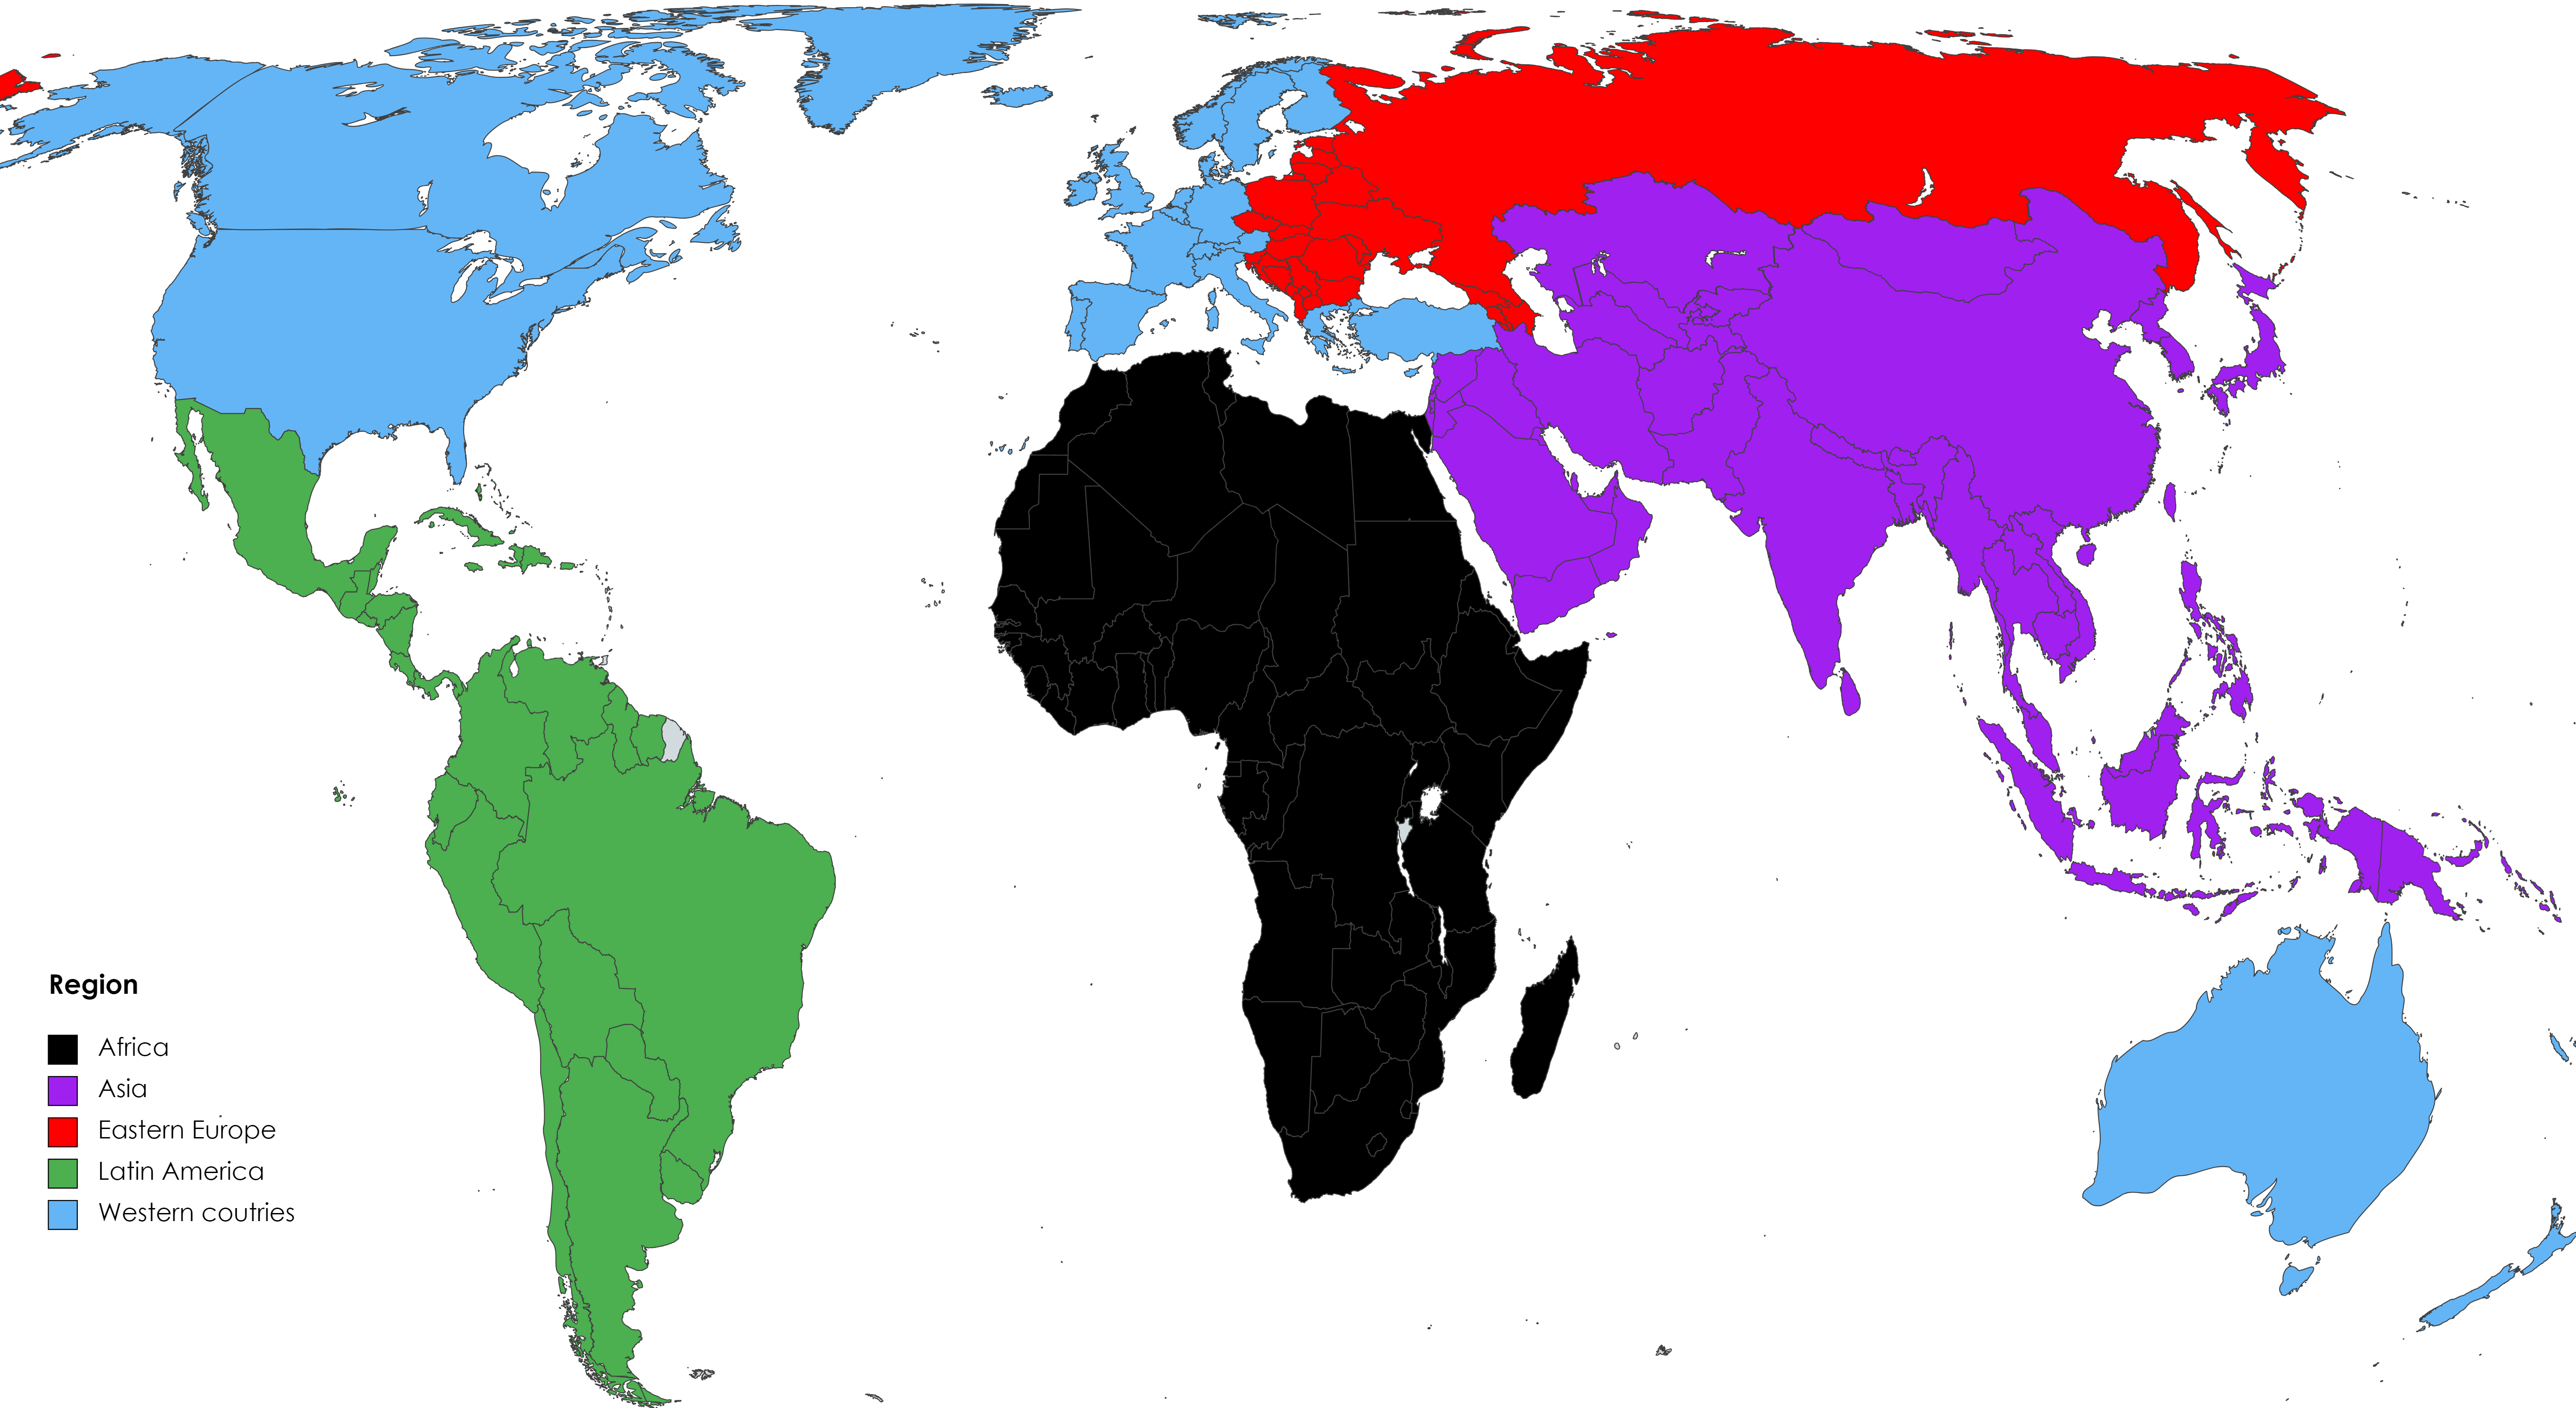
\includegraphics[width=.9\textwidth]{../figures/region_groupings.png}
\end{figure}
\fi

% Shared section: the Fabre (2025) survey experiment
\subsection{A survey experiment on question wording and scale}\label{subsec:fabre}

Gallup and the WVS differ in many respects. Gallup asks the Cantril ladder on a 0--10 scale, the WVS life satisfaction on a 1--10 scale. Gallup relies on a centralized, standardized design, with about 1,000 respondents per country every year, interviewed by telephone in high-income countries and face-to-face elsewhere; the WVS is fielded every five years or so by national teams, mostly face-to-face, with sampling designs, modes and survey years that vary across countries. These differences fall into two categories that could explain why the two datasets disagree: the question (wording and scale) and everything else---sampling frames, interview modes, questionnaire context, translations, and survey years, which I refer to as \textit{samples} in a broad sense. To separate the two, I embedded a randomized experiment in an original survey \citep{fabre_public_2025}. The survey was conducted online between April 15 and July 3, 2025, by Bilendi (or Kantar in Saudi Arabia) on \nFabre respondents in \nFabreCountries high-income countries: the United States (3,000), Japan (2,000), Saudi Arabia (1,000), Germany (1,048), the United Kingdom (826), France (798), Italy (756), Spain (603), Poland (500) and Switzerland (469).\footnote{The survey also covered Russia, where the well-being question was censored.} Samples were stratified with quotas on gender, age, income, education, region and urbanicity,\footnote{Quota variables also included race in the U.S. and citizenship in Saudi Arabia.} and results are reweighted to match population frequencies along these dimensions (with weights trimmed between 0.25 and 4).

Toward the end of the questionnaire, after questions on global policies, each respondent was randomly assigned to one of four versions of the life-evaluation question:
\begin{itemize}
    \item \textit{Ladder 0--10} (Gallup's original): the Cantril ladder question quoted in Section~\ref{subsec:gallup}, with steps numbered from 0 (\textit{Worst possible}) to 10 (\textit{Best possible});
    \item \textit{Ladder 1--10}: same wording, with steps numbered from 1 to 10;
    \item \textit{Satisfaction 0--10}: the WVS question quoted in Section~\ref{subsec:wvs}, with answers from 0 (\textit{Completely dissatisfied}) to 10 (\textit{Completely satisfied});
    \item \textit{Satisfaction 1--10} (WVS's original): same wording, with answers from 1 to 10.
\end{itemize}
This $2 \times 2$ design identifies the effect of wording (ladder vs.\ satisfaction) and scale (0--10 vs.\ 1--10), and their interaction, holding the sample, mode, context and time constant. Within each country, each branch receives around 25\% of respondents.


\section{Results}\label{sec:results}
\subsection{The discrepancy}\label{subsec:global_gap}
% Shared section: why do Gallup and the WVS disagree? Wording vs. sampling

Restricting both datasets to the \nCommon country-years (\nCommonCountries countries) observed by both surveys the same year, log GDP explains \RtwoCommonGallup of the variance of Gallup's mean ladder but only \RtwoCommonWVS of WVS mean satisfaction, and income accounts for \shareIncomeCommonGallup\% of the variance explained jointly with region in Gallup against \shareIncomeCommonWVS\% in the WVS (the share of the $R^2$ of a regression on log GDP and five region dummies attributed to income by the Shapley decomposition; see the companion paper \todo{cite}). The discrepancy is thus not due to different country coverage. The gap between the two datasets decreases strongly with GDP (Figure~\ref{fig:gap_gdp}): the slope is \slopeGapGDP per unit of $\log_{10}$ GDP (s.e.\ \seSlopeGapGDP, clustered by country), with WVS answers exceeding Gallup answers by around two points in low-income countries, against less than half a point in high-income countries.

\begin{figure}[htbp]
    \centering
    \caption{WVS satisfaction minus Gallup ladder in the same country-year, by GDP per capita.}\label{fig:gap_gdp}
    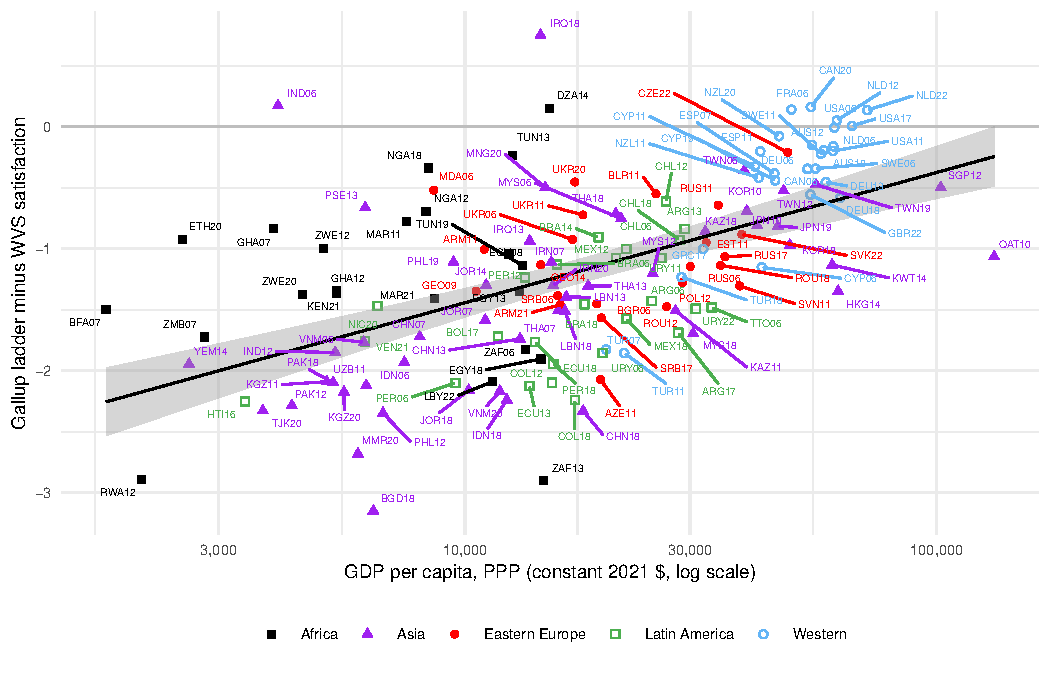
\includegraphics[width=.9\textwidth]{../figures/main/gap_gallup_wvs_vs_gdp.pdf}
    \begin{minipage}{.9\textwidth}\footnotesize \textit{Note:} Mean answers on native scales (WVS: 1--10; Gallup: 0--10), \nCommon country-years observed by both surveys. Line: OLS fit with 95\% confidence band.\end{minipage}
\end{figure}

The two datasets differ in their question (ladder 0--10 vs.\ satisfaction 1--10) and in their samples in the broad sense defined in Section~\ref{subsec:fabre}. The experiment allows me to measure how much of the discrepancy the question accounts for: first for the relation between income and well-being, which is the object of this paper (Section~\ref{subsec:ten_countries}), then for levels (Section~\ref{subsec:experiment}).

\subsection{Does wording explain the discrepancy? Evidence from ten countries}\label{subsec:ten_countries}

The ten countries of the experiment provide a direct test. Since the object of interest is national well-being, the unit of observation is the country: for each question variant, I compute the mean answer in each country and regress it on log GDP per capita across the ten countries, as for the Gallup and WVS country means (Table~\ref{tab:ten_countries} and Figure~\ref{fig:fabre_gdp}). Each country thus has the same weight, whatever its sample size. For Gallup and the WVS, I use the latest WVS or EVS survey of each country (2017--2022, except Saudi Arabia, 2003) and the Gallup data of the same year (or the closest year, at most three years apart). Confidence intervals come from a bootstrap that resamples respondents in the three surveys.

I first compare $R^2$, which directly measure the predictive capacity of GDP per capita. In the past data, the ten countries reproduce the global discrepancy: log GDP explains \RtwoTenGallup (95\% CI [\decompLowRGallup; \decompHighRGallup]) of the cross-country variance of Gallup's ladder but only \RtwoTenWVS ([\decompLowRWvs; \decompHighRWvs]) of WVS satisfaction. Asked to the same online sample, the two original questions reproduce much of this contrast: log GDP explains \RtwoTenFabreLadder ([\decompLowRFabreLadder; \decompHighRFabreLadder]) of the variance of the ladder 0--10 but \RtwoTenFabreSatisfaction ([\decompLowRFabreSatisfaction; \decompHighRFabreSatisfaction]) of satisfaction 1--10. Pooling both scales of each wording, the $R^2$ is \RtwoTenFabreLadderPooled for the ladder and \RtwoTenFabreSatisfactionPooled for satisfaction. The wording thus accounts for \decompShareRWordingPooled (95\% CI [\decompLowShareRWordingPooled; \decompHighShareRWordingPooled]) of the Gallup--WVS difference in $R^2$ (\decompShareRWording with the two original variants only, [\decompLowShareRWording; \decompHighShareRWording]), and samples for the rest. In other words, the new data lie midway between Gallup and the WVS. Pooling the four variants, log GDP explains \RtwoTenFabreAll of the variance, and income accounts for \shareIncomeTenFabreAll of the variance explained jointly with region, halfway between Gallup (\shareIncomeTenGallup) and the WVS (\shareIncomeTenWVS). The two crossed variants, which combine the wording of one survey with the scale of the other (ladder 1--10 and satisfaction 0--10), also yield intermediate results, with $R^2$ of \RtwoTenFabreLadderOneTen and \RtwoTenFabreSatisfactionZeroTen and slopes of \slopeTenFabreLadderOneTen and \slopeTenFabreSatisfactionZeroTen. Only Gallup's original variant yields a high $R^2$, so that with ten countries, the effect of the wording cannot be clearly separated from that of the scale.

\begin{table}[htbp]
    \centering
    \caption{Relation between GDP per capita and national well-being in the ten countries of the experiment: past vs.\ new data.}\label{tab:ten_countries}
    \begin{adjustbox}{max width=\textwidth}
    \begin{tabular}{lccccc}
\toprule
Data & Slope on $\log_{10}$ GDP & s.e. & $R^2$ income & $R^2$ region & Share due to income \\
\midrule
Gallup (ladder 0--10) & 4.20 & 0.80 & 0.75 & 0.29 & 0.78 \\
WVS/EVS (satisfaction 1--10) & 1.36 & 1.44 & 0.16 & 0.34 & 0.35 \\
\midrule
Fabre 2025: ladder 0--10 & 4.35 & 1.05 & 0.76 & 0.14 & 0.91 \\
Fabre 2025: ladder 1--10 & 2.57 & 1.36 & 0.33 & 0.50 & 0.36 \\
Fabre 2025: satisfaction 0--10 & 3.21 & 2.03 & 0.23 & 0.36 & 0.35 \\
Fabre 2025: satisfaction 1--10 & 4.05 & 2.09 & 0.31 & 0.29 & 0.52 \\
\bottomrule
\end{tabular}

    \end{adjustbox}
    \begin{minipage}{\textwidth}\footnotesize \textit{Note:} OLS across the \nDecompCountries countries of the experiment, one observation per country. Gallup and WVS/EVS: latest WVS/EVS survey and Gallup the same year, GDP of that year. Fabre (2025): mean answer by variant (native scale), GDP of 2025; ``both scales'' and ``all four variants'': average of the variant means, 1--10 answers being linearly stretched to 0--10. 95\% CI of $R^2$: bootstrap resampling respondents. Standard errors of slopes robust to heteroskedasticity (HC1). $R^2$ region: $R^2$ of the regression on region dummies (Western, Asia, Eastern Europe). Share due to income: Shapley share of the $R^2$ of the regression on log GDP and region attributed to income.\end{minipage}
\end{table}

Slopes tell a different story. Both questions yield an income gradient close to Gallup's (\slopeTenGallup): \slopeTenFabreLadder with the ladder and \slopeTenFabreSatisfaction with the satisfaction question (\slopeTenFabreLadderPooled and \slopeTenFabreSatisfactionPooled when pooling scales), whereas the WVS gradient is three times flatter (\slopeTenWVS). The part of the Gallup--WVS difference in slopes that is not due to the question is \SlopeDiffinDiff (95\% CI [\SlopeDiffinDiffLow; \SlopeDiffinDiffHigh]). How can the satisfaction question yield a lower $R^2$ but the same slope as the ladder? With a single regressor, $R^2 = \beta^2 \mathrm{var}(x)/\mathrm{var}(y)$: for a given slope, the $R^2$ is lower when country means are more dispersed around the income gradient. The satisfaction question does not weaken the gradient, but it produces larger country-specific deviations from it---most visibly in Japan, whose mean satisfaction (\meanSatisfactionJPN on the 1--10 scale) is \gapSatisfactionJPN points below that of any other country despite its high income, whereas its mean ladder (\meanLadderJPN) is only \gapLadderJPN points below the next lowest (Appendix Table~\ref{tab:decomposition_country}). These country-specific deviations are precisely what region captures in the WVS. By contrast, the flat WVS gradient is specific to its samples.

I give more weight to the $R^2$ than to the slopes, because the question of this paper is the predictive capacity of GDP per capita, which the $R^2$ measures. Taken together, the results suggest that the wording accounts for about half of the difference in predictive capacity between Gallup and the WVS, through larger country-specific deviations in answers to the satisfaction question, while differences between samples account for the other half and for most of the difference in the income gradient. Two caveats apply. First, the bootstrap confidence intervals reflect the sampling of respondents and treat the ten countries as given; with only ten countries, $R^2$ and slopes are imprecise (Table~\ref{tab:ten_countries} reports the standard errors of slopes across countries) and sensitive to individual countries. For instance, excluding Japan raises the $R^2$ of Gallup to \RtwoGallupNoJPN and lowers the share of the Gallup--WVS difference in $R^2$ due to wording to \shareRtwoWordingPooledNoJPN. Second, the decompositions between income and region are of limited use here, since seven out of the ten countries are Western.

\begin{figure}[htbp]
    \centering
    \caption{Mean life evaluation vs.\ GDP per capita (PPP), by question variant, Fabre (2025).}\label{fig:fabre_gdp}
    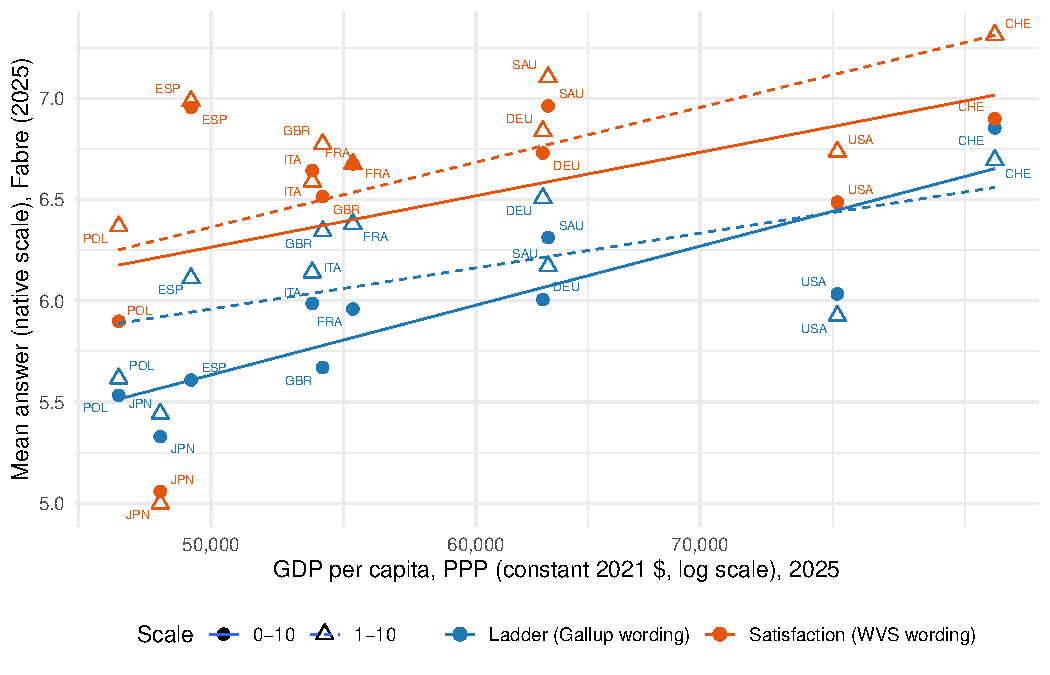
\includegraphics[width=.9\textwidth]{../figures/main/fabre_mean_vs_gdp_ppp.pdf}
    \begin{minipage}{.9\textwidth}\footnotesize \textit{Note:} Mean answer on the native scale of each variant (0--10 or 1--10), ten countries surveyed in 2025. Colors: wording; shapes and line types: scale. Lines: OLS fits by variant.\end{minipage}
\end{figure}

Can the question explain the global pattern, where the gap between WVS and Gallup answers is largest in low-income countries? To gauge this, I estimate the question effect as a linear function of log GDP across the ten countries, and I convert each WVS country mean into a ladder-equivalent by subtracting the question effect predicted for its GDP. As the question effect is not significantly related to GDP within the experiment (slope \slopeQuestionGDP, s.e.\ \seSlopeQuestionGDP), which is unsurprising given the narrow range of GDP among the ten countries, this adjustment raises the $R^2$ of WVS satisfaction on log GDP only from \RtwoCommonWVS to \RtwoAdjustedWVS, far from Gallup's \RtwoCommonGallup. This adjustment only captures level differences that vary with GDP, not the additional country-specific dispersion that the satisfaction question produces in the experiment. Moreover, the experiment cannot rule out that the wording effect is much larger in low-income countries---for instance if the ``best possible life'' evokes material comparisons more strongly where material deprivation is widespread. Nothing in the high-income evidence points in that direction, though: within countries, the ladder does not steepen the individual income gradient (Section~\ref{subsec:experiment}).

\subsection{Wording and the levels of well-being}\label{subsec:experiment}

Although levels matter less than correlations for our question, the experiment also explains why the WVS yields higher levels than Gallup. Appendix Table~\ref{tab:fabre_regressions} reports regressions of the answer on the randomized treatments, with country fixed effects, survey weights and heteroskedasticity-robust standard errors. The ladder wording shifts answers by \effectLadder points on average (s.e.\ \seLadder): respondents rate their lives lower on the ``best possible life'' ladder than when asked how satisfied they are, in line with evidence that the ladder evokes power and wealth more than life satisfaction does \citep{nilsson_cantril_2024}. Answers on the 1--10 scale are \effectScale points higher than on the 0--10 scale (s.e.\ \seScale). Once 1--10 answers are linearly stretched to 0--10 with $x \mapsto (x-1) \times 10/9$, which maps 1 to 0 and 10 to 10, the scale effect becomes \effectScaleZeroTen: the stretch lowers each answer $x$ by $(10-x)/9$, i.e.\ by about 0.4 points at the average answer. Wording and scale do not interact. The wording effect varies markedly across countries (Figure~\ref{fig:decomposition}; $\chi^2(9) = \chiHeterogeneityWording$, $p \pHeterogeneityWording$). Japan is the exception: it is the only country where the ladder yields \textit{higher} answers than the satisfaction question (by \wordingJPN points); elsewhere, the wording effect ranges from \wordingMin (Spain) to \wordingMaxNegative points. Finally, the ladder does not steepen the income gradient \textit{within} countries: the interaction between the ladder wording and the respondent's income quartile is \interactionLadderIncome ($p \pInteractionLadderIncome$), against a gradient of \gradientIncomeSatisfaction points per quartile.

To relate these effects to the Gallup--WVS gap, I define for each country $c$ the observed gap $D_c = W_c - G_c$, where $W_c$ is mean satisfaction in the WVS and $G_c$ the mean ladder in Gallup the same year (as in Section~\ref{subsec:ten_countries}), and the question effect $Q_c = F_c(\text{satisfaction 1--10}) - F_c(\text{ladder 0--10})$, the difference between the mean answers to the two original variants in the experiment, measured on the same sample. The residual $R_c = D_c - Q_c$ is the part of the gap due to samples in the broad sense. On average, WVS answers exceed Gallup answers by $D = \decompMeanGap$ points, and the question effect is even larger: $Q = \decompMeanQuestion$ points (Appendix Tables~\ref{tab:decomposition_country} and \ref{tab:decomposition_summary}). The question thus fully accounts for the higher level of WVS answers in high-income countries, and the residual is small ($R = \decompMeanResidual$, 95\% CI [\decompLowMeanResidual; \decompHighMeanResidual]). Since the two components move in opposite directions, another way to summarize the level difference is to compare the size of the two movements: the question accounts for $|\bar Q|/(|\bar Q|+|\bar R|) = \decompShareAbsQuestion$ (95\% CI [\decompLowShareAbsQuestion; \decompHighShareAbsQuestion]) of the gross difference in levels.

\begin{figure}[htbp]
    \centering
    \caption{Observed WVS--Gallup gap, question effect and residual by country.}\label{fig:decomposition}
    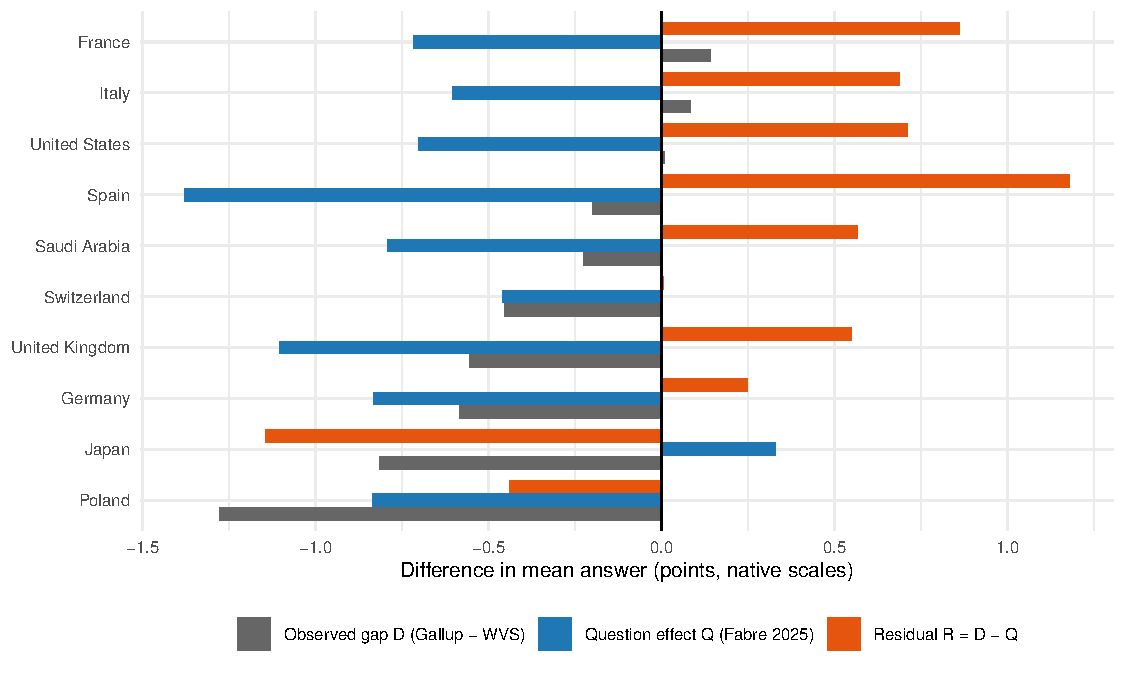
\includegraphics[width=.9\textwidth]{../figures/main/decomposition_by_country.pdf}
    \begin{minipage}{.9\textwidth}\footnotesize \textit{Note:} $D$: mean satisfaction (WVS/EVS, 1--10) minus mean ladder (Gallup, 0--10), same year. $Q$: mean answer to satisfaction 1--10 minus mean answer to ladder 0--10, Fabre (2025). $R = D - Q$.\end{minipage}
\end{figure}

The question effect does not, however, explain why the gap varies across countries. Since $D_c = Q_c + R_c$, the cross-country variance of the gap splits into $\mathrm{var}(D) = \mathrm{cov}(D,Q) + \mathrm{cov}(D,R)$. The share attributable to the question, $\mathrm{cov}(D,Q)/\mathrm{var}(D)$, is only \decompVarShareQuestion (95\% CI [\decompLowVarShareQuestion; \decompHighVarShareQuestion]): countries with a larger question effect do not have a larger gap. Accordingly, predicting each country's Gallup mean by subtracting its own question effect $Q_c$ from its WVS mean does worse (root mean squared error: \decompRmsePredictionGallup) than simply subtracting the average gap (\decompRmseNaive). Samples asked the same question also differ markedly. Gallup respondents (2023--2025) rate their lives \meanSampleEffectGallup points higher on the ladder 0--10 than online respondents in 2025, and WVS respondents \meanSampleEffectWVS points higher on satisfaction 1--10 (even in the United States, where the 2017 WVS was itself conducted online: \sampleEffectUSWVS points). And in the \nEVSvsWVS countries surveyed separately by the EVS and the WVS in 2017--2022, with the same question, mean satisfaction differs by \meanAbsDiffEVSWVS points on average (up to \maxAbsDiffEVSWVS).

\subsection{Which dataset has more representative samples?}\label{subsec:data_quality}

If samples matter, which dataset is closer to the truth? There is no clear-cut argument in favor of either dataset, nor of the online sample used in the experiment. Gallup applies a centralized, standardized design: probability samples of about 1,000 adults per year, drawn by random-digit dialing where telephone coverage is high and by multistage area sampling elsewhere, with random selection of the respondent within the household and post-stratification weights on gender, age and, where possible, education \citep{gallup_methodology_2023}. But its samples are small; its face-to-face samples select households by random route, with replacement of non-responding households; response rates are not published; interviews switched from face-to-face to telephone during the pandemic; and in 2023, a fifth of the interviews in 27 high-income countries came from web panels, most of them opt-in \citep{gallup_methodology_2023}. Its subgroup estimates have also been questioned \citep{blanchflower_gallup_2024}. Besides, Gallup microdata are not public, so that the representativeness of its samples cannot be assessed independently; lacking quotas, its samples could under-represent hard-to-reach groups such as less educated or rural people. The WVS requires probability samples of at least 1,200 respondents but allows quota selection at the last stage, and its sampling designs, modes and survey years vary across countries \citep{wvs_rules_wave8}. Tests flagging near-duplicate interviews (pairs of respondents giving identical answers to almost all questions, a possible sign of fabrication) in international survey programs \citep{kuriakose_dont_2016} have been disputed \citep{pew_data_2016}. Finally, online panels exclude people without internet access, and quotas on observable characteristics do not guarantee representativeness in unobservable ones.

I test the representativeness of WVS/EVS samples directly (Appendix Table~\ref{tab:representativeness}). Compared with population benchmarks \citep{barro_new_2013,worldbank_wdi_2026}, WVS samples over-represent tertiary-educated adults (aged 25 and over) by a median factor of \ratioTertiaryLow in countries with a GDP per capita below 10,000 dollars, against \ratioTertiaryHigh in countries above 30,000 dollars (\nCompositionSurveys surveys). They also over-represent urban residents in poorer countries (median ratio \ratioUrbanLow vs.\ \ratioUrbanHigh) and under-represent people aged 65 or more (\ratioOldLow vs.\ \ratioOldHigh). The internal criterion of \citet{kohler_surveys_2007}---women should make up half of married or cohabiting respondents---is violated at the 5\% level in \shareGenderFlag\% of surveys. WVS samples are thus less representative in poorer countries, as noted by \citet{deaton_income_2008}, which is where their gap with Gallup is largest. However, correcting these observable imbalances has little effect. Controlling for log GDP, the over-representation of the tertiary-educated does not predict the gap (coefficient \coefTertiaryGap, s.e.\ \seTertiaryGap, $p \pTertiaryGap$), and reweighting each WVS sample to the benchmark share of tertiary-educated adults barely changes its relation with income: in the country-years also covered by Gallup, the $R^2$ of mean satisfaction on log GDP goes from \RtwoCommonWVSraw to \RtwoCommonWVSeduAdj, against \RtwoCommonGallupSub for Gallup. The discrepancy thus stems from unobserved differences in who responds, how, and in which context, which the available evidence does not allow me to attribute to one dataset rather than the other.


\section{Discussion}\label{sec:discussion}
% Shared section: interpretation and limitations of the wording vs. sampling decomposition
The experiment shows that the question matters in two ways. It matters for levels: the Cantril ladder yields lower answers than the WVS life-satisfaction question, and this difference fully accounts for the lower average level of Gallup data in high-income countries. And it matters for predictive capacity: asked to the same sample, the ladder is better predicted by GDP, because the satisfaction question produces larger country-specific deviations from the income gradient. This reproduces about half of the Gallup--WVS difference in $R^2$. But the question does not explain the flat income gradient of the WVS, nor the cross-country pattern of the Gallup--WVS gap in levels, which reflect differences between samples in the broad sense: sampling frames, interview modes \citep{dolan_happy_2016,conti_survey_2011}, questionnaire context \citep{deaton_financial_2012,deaton_understanding_2016}, translations, and time.

Several limitations should be kept in mind. First, the experiment covers only ten high-income countries, whereas the gap varies most across income levels, and where both Gallup and the WVS mostly interview face-to-face; only an experiment in low- and middle-income countries can settle this. Second, the residual lumps together several factors that the design cannot separate; in particular, the question effect was measured online, toward the end of the questionnaire, and may differ from the effect that would be obtained at the beginning of an interview conducted face-to-face or by phone. Third, with ten countries, cross-country statistics are imprecise. Fourth, the comparison with past data assumes that the question effect measured in 2025 applies to the surveys of 2017--2022 (2003 for Saudi Arabia).


Finally, online panel respondents report markedly lower well-being than Gallup and WVS respondents asked the same question, a sample and mode effect that deserves attention in its own right as online panels become common in well-being research.

\section{Conclusion}\label{sec:conclusion}

The Gallup World Poll and the World Values Survey disagree on how strongly national well-being is related to income. A survey experiment in ten high-income countries shows that both their questions and their samples contribute to this discrepancy. Asked to the same sample, the Cantril ladder is better predicted by GDP than the life-satisfaction question, reproducing about half of the Gallup--WVS difference in predictive capacity: the new data lie midway between the two datasets. But both questions yield an income gradient close to Gallup's, whereas the WVS gradient is much flatter; and the question fully accounts for the lower level of Gallup answers, but not for the cross-country pattern of the gap.

This has two implications. First, the Cantril ladder and the life-satisfaction question are not interchangeable: they differ in level and, among countries at similar income levels, in the ranking of countries, so that cross-country conclusions should be checked across questions as well as datasets. Second, the available evidence does not establish that one dataset has more representative samples than the other. The two surveys disagree most in low-income countries, where there is not yet evidence on which is closer to the truth. Replicating the experiment face-to-face in low- and middle-income countries, with official translations and at the beginning of the interview, is the natural next step.

\section*{Declaration of generative AI and AI-assisted technologies in the writing process}
During the preparation of this work the author used Claude Opus 5.5 to write analysis code and draft parts of the manuscript. After using this tool, the author reviewed and edited the code and content created by AI as needed and takes full responsibility for the content of the publication.

\bibliography{wellbeing}

\clearpage
\appendix
\section{Additional results}\label{app:additional}
\renewcommand{\thetable}{A\arabic{table}}
\renewcommand{\thefigure}{A\arabic{figure}}
\setcounter{table}{0}
\setcounter{figure}{0}

\begin{table}[htbp]
    \centering
    \caption{Effects of question wording and scale on life evaluation, Fabre (2025) survey experiment.}\label{tab:fabre_regressions}
    \begin{adjustbox}{max width=\textwidth}
    
\begingroup
\centering
\begin{tabular}{lcccccc}
   \tabularnewline \midrule \midrule
   Dependent Variables: & \multicolumn{2}{c}{Answer} & Answer (0--10 equiv.) & Satisfied (6+) & \multicolumn{2}{c}{Answer (0--10 equiv.)}\\
   Model:                                                                         & (1)            & (2)            & (3)            & (4)            & (5)            & (6)\\  
   \midrule
   \emph{Variables}\\
   Ladder wording (Gallup)                                                        & -0.451$^{***}$ & -0.455$^{***}$ & -0.456$^{***}$ & -0.088$^{***}$ & -0.464$^{***}$ & -0.494$^{**}$\\   
                                                                                  & (0.046)        & (0.067)        & (0.067)        & (0.013)        & (0.123)        & (0.172)\\   
   Scale 1--10                                                                    & 0.137$^{**}$   & 0.132          & -0.260$^{***}$ & -0.008         & -0.276$^{***}$ & -0.540$^{**}$\\   
                                                                                  & (0.046)        & (0.068)        & (0.072)        & (0.013)        & (0.046)        & (0.182)\\   
   Ladder wording (Gallup) $\times$ Scale 1--10                                   &                & 0.008          & -0.041         & 0.028          &                & 0.055\\   
                                                                                  &                & (0.092)        & (0.097)        & (0.019)        &                & (0.247)\\   
   Income quartile (1--4)                                                         &                &                &                &                & 0.689$^{***}$  & 0.635$^{***}$\\   
                                                                                  &                &                &                &                & (0.031)        & (0.043)\\   
   Income quartile (1--4) $\times$ Ladder wording (Gallup)                        &                &                &                &                & -0.004         & 0.009\\   
                                                                                  &                &                &                &                & (0.042)        & (0.058)\\   
   Income quartile (1--4) $\times$ Scale 1--10                                    &                &                &                &                &                & 0.106\\   
                                                                                  &                &                &                &                &                & (0.061)\\   
   Income quartile (1--4) $\times$ Ladder wording (Gallup) $\times$ Scale 1--10   &                &                &                &                &                & -0.022\\   
                                                                                  &                &                &                &                &                & (0.083)\\   
   \midrule
   \emph{Fixed-effects}\\
   Country                                                                        & Yes            & Yes            & Yes            & Yes            & Yes            & Yes\\  
   \midrule
   \emph{Fit statistics}\\
   Observations                                                                   & 11,000         & 11,000         & 11,000         & 11,000         & 11,000         & 11,000\\  
   R$^2$                                                                          & 0.05681        & 0.05681        & 0.05942        & 0.04208        & 0.15976        & 0.16024\\  
   \midrule \midrule
   \multicolumn{7}{l}{\emph{Heteroskedasticity-robust standard-errors in parentheses}}\\
   \multicolumn{7}{l}{\emph{Signif. Codes: ***: 0.001, **: 0.01, *: 0.05}}\\
\end{tabular}
\par\endgroup



    \end{adjustbox}
    \begin{minipage}{\textwidth}\footnotesize \textit{Note:} OLS with country fixed effects, survey weights (normalized within country) and heteroskedasticity-robust standard errors in parentheses. \textit{Ladder wording}: Cantril ladder (vs.\ WVS life satisfaction). \textit{Scale 1--10}: answers from 1 to 10 (vs.\ 0 to 10). In columns 3, 5 and 6, 1--10 answers are linearly stretched to 0--10. Columns 5 and 6 interact the treatments with the respondent's income quartile within their country; in column 6, the interaction between income and wording is \interactionLadderIncomeFull ($p \pInteractionLadderIncomeFull$) and the triple interaction is \tripleInteraction ($p \pTripleInteraction$). * $p<.05$, ** $p<.01$, *** $p<.001$. \hfill(Back~to~Section~\ref{subsec:experiment}.)\end{minipage}
\end{table}

\begin{table}[htbp]
    \centering
    \caption{Decomposition of the WVS--Gallup gap by country.}\label{tab:decomposition_country}
    \begin{adjustbox}{max width=\textwidth}
    \begin{tabular}{lllccccccc}
\toprule
Country & Year WVS/EVS (Gallup) & Survey: mode & Gallup & WVS/EVS & Gap $D$ & Ladder 0--10 & Satisf. 1--10 & Question effect $Q$ & Residual $R$ \\ & & & (1) & (2) & (1)$-$(2) & \multicolumn{2}{c}{Fabre (2025)} & & $D-Q$ \\
\midrule
Poland & 2017 & EVS: CAPI & 6.28 & 7.56 & \ensuremath{-}1.28 & 5.53 & 6.37 & \ensuremath{-}0.84 & \ensuremath{-}0.44 \\
Spain & 2017 & EVS: CAPI & 6.47 & 7.49 & \ensuremath{-}1.02 & 5.61 & 6.99 & \ensuremath{-}1.38 & 0.36 \\
Japan & 2019 & WVS: Mail & 5.94 & 6.76 & \ensuremath{-}0.82 & 5.33 & 5.00 & 0.33 & \ensuremath{-}1.15 \\
Italy & 2018 & EVS: CAPI & 6.69 & 7.28 & \ensuremath{-}0.59 & 5.99 & 6.59 & \ensuremath{-}0.60 & 0.01 \\
Germany & 2018 & WVS: CAPI & 7.15 & 7.74 & \ensuremath{-}0.58 & 6.01 & 6.84 & \ensuremath{-}0.83 & 0.25 \\
United Kingdom & 2022 & WVS: CAPI/Web/Mail & 6.76 & 7.32 & \ensuremath{-}0.56 & 5.67 & 6.77 & \ensuremath{-}1.10 & 0.55 \\
France & 2018 & EVS: CAPI & 6.79 & 7.26 & \ensuremath{-}0.47 & 5.96 & 6.68 & \ensuremath{-}0.72 & 0.25 \\
Switzerland & 2017 & EVS: Web/Mail/CAPI & 7.58 & 8.02 & \ensuremath{-}0.43 & 6.85 & 7.31 & \ensuremath{-}0.46 & 0.03 \\
Saudi Arabia & 2003 (2006) & WVS: Face-to-face & 7.06 & 7.28 & \ensuremath{-}0.23 & 6.31 & 7.10 & \ensuremath{-}0.79 & 0.57 \\
United States & 2017 & WVS: Web/Phone & 7.23 & 7.22 & 0.01 & 6.03 & 6.74 & \ensuremath{-}0.70 & 0.71 \\
\bottomrule
\end{tabular}

    \end{adjustbox}
    \begin{minipage}{\textwidth}\footnotesize \textit{Note:} Mean answers on native scales (Gallup and ladder: 0--10; WVS/EVS and satisfaction: 1--10); columns (3) and (4): Fabre (2025). The Gallup year is given in parentheses when it differs from the WVS year. Survey: mode: source of the WVS/EVS data and main interview mode(s) (CAPI: computer-assisted personal interviews). \hfill(Back~to~Section~\ref{subsec:experiment}.)\end{minipage}
\end{table}

\begin{table}[htbp]
    \centering
    \caption{Decomposition of the WVS--Gallup gap: summary.}\label{tab:decomposition_summary}
    \begin{adjustbox}{max width=\textwidth}
    \begin{tabular}{lc}
\toprule
Statistic & Estimate [95\% bootstrap CI] \\
\midrule
Mean gap $D$ (Gallup $-$ WVS) & \ensuremath{-}0.60 [\ensuremath{-}0.64; \ensuremath{-}0.55] \\
Mean question effect $Q$ (wording + scale) & \ensuremath{-}0.71 [\ensuremath{-}0.84; \ensuremath{-}0.56] \\
Mean residual $R$ (sampling, mode, context) & 0.11 [\ensuremath{-}0.04; 0.26] \\
\midrule
Share of mean gap due to question ($\bar Q/\bar D$) & 1.19 [0.94; 1.45] \\
Share of gross level difference due to question ($|\bar Q|/(|\bar Q|+|\bar R|)$) & 0.86 [0.76; 0.99] \\
Same, country average ($\overline{|Q_c|/(|Q_c|+|R_c|)}$) & 0.69 [0.56; 0.72] \\
\midrule
Share of cross-country variance of $D$ due to $Q$ ($\mathrm{cov}(D,Q)/\mathrm{var}(D)$) & 0.11 [\ensuremath{-}0.33; 0.55] \\
Share of cross-country variance of $D$ due to $R$ & 0.89 [0.45; 1.33] \\
Mean absolute gap $|D|$ & 0.60 [0.56; 0.65] \\
Mean absolute residual $|R|$ & 0.43 [0.33; 0.60] \\
Correlation between $D$ and $Q$ & 0.09 [\ensuremath{-}0.26; 0.41] \\
\midrule
Mean gap, share satisfied (6+) & \ensuremath{-}0.07 [\ensuremath{-}0.08; \ensuremath{-}0.06] \\
Mean question effect, share satisfied (6+) & \ensuremath{-}0.11 [\ensuremath{-}0.14; \ensuremath{-}0.08] \\
Variance share due to $Q$, share satisfied & 0.04 [\ensuremath{-}0.33; 0.45] \\
\bottomrule
\end{tabular}

    \end{adjustbox}
    \begin{minipage}{\textwidth}\footnotesize \textit{Note:} \nDecompCountries countries. 95\% confidence intervals from 1,000 bootstrap replications resampling respondents within country $\times$ variant (Fabre) and within country (WVS). For Gallup, only the distribution of answers is available: in each country, the numbers of respondents giving each answer (0 to 10) are redrawn from a multinomial distribution with the observed shares and sample size, which is equivalent to resampling respondents. \hfill(Back~to~Section~\ref{subsec:experiment}.)\end{minipage}
\end{table}

\begin{table}[htbp]
    \centering
    \caption{Representativeness of WVS/EVS samples: sample shares relative to population benchmarks.}\label{tab:representativeness}
    \begin{adjustbox}{max width=\textwidth}
    \begin{tabular}{lcccccc}
\toprule
Measure & Surveys & \multicolumn{4}{c}{Median} & Correlation \\ & & All & GDP $<$ 10k & 10--30k & $>$ 30k & with log GDP \\
\midrule
Tertiary education, 25+ (ratio sample/benchmark) & 295 & 1.18 & 1.98 & 1.18 & 1.05 & \ensuremath{-}0.40 \\
Urban (ratio sample/benchmark) & 76 & 1.44 & 2.19 & 1.45 & 1.22 & \ensuremath{-}0.69 \\
Aged 65+ (ratio sample/benchmark) & 335 & 0.90 & 0.64 & 0.88 & 1.01 & 0.33 \\
Women among married respondents $-$ 0.5 & 337 & 0.01 & \ensuremath{-}0.00 & 0.01 & 0.01 & 0.19 \\
\bottomrule
\end{tabular}

    \end{adjustbox}
    \begin{minipage}{\textwidth}\footnotesize \textit{Note:} One observation per WVS or EVS survey. Ratios: weighted sample share divided by the population share, medians across surveys (a ratio above 1 indicates over-representation). Benchmarks (World Bank WDI): share of the population aged 25+ with at least short-cycle tertiary education (UNESCO), or with complete or incomplete tertiary education \citep{barro_new_2013} before 2011; urban population share (national definitions; sample: urban and peri-urban respondents, waves 4, 5 and 7 only); share aged 65+ among the population aged 15+ (sample: 65+ among respondents, usually 18+). Women among married: unweighted share of women among married or cohabiting respondents minus 0.5. Correlations with log GDP per capita (PPP) of the log ratios (or of the deviation). \hfill(Back~to~Section~\ref{subsec:data_quality}.)\end{minipage}
\end{table}

\end{document}
